\documentclass{article}
\usepackage[margin=1in]{geometry}
\usepackage{graphicx}
\usepackage{enumitem}
\usepackage[toc,page]{appendix}
\usepackage{amsfonts}
\usepackage{amsmath}
\usepackage{amsthm}
\usepackage{commath}
\usepackage{color}

\title{FLASH Orchestration Runtime Design}

% No automatic indenting
\setlength\parindent{0pt}

% Set spacing between items in itemize/enumerate
\setlist{itemsep=1pt}

\newcommand{\N}                 {{\mathbb N}}
\newcommand{\Z}                 {{\mathbb Z}}
\newcommand{\Q}                 {{\mathbb Q}}
\newcommand{\R}                 {{\mathbb R}}
\newcommand{\C}                 {{\mathbb C}}
\newcommand{\F}                 {{\mathbb F}}

\newcommand{\SetuptimeParam}[1] {\textcolor{red}{#1}}
\newcommand{\RuntimeParam}[1]   {\textcolor{blue}{#1}}
\newcommand{\ComposerKey}[1]    {\textcolor{cyan}{#1}}

\newcommand{\TeamStarting}      {\textsc{TeamStarting}}
\newcommand{\TeamIdle}          {\textsc{TeamIdle}}
\newcommand{\TeamRunningOpen}   {\textsc{TeamRunningOpen}}
\newcommand{\TeamRunningClosed} {\textsc{TeamRunningClosed}}
\newcommand{\TeamRunningNoMoreWork} {\textsc{TeamRunningNoMoreWork}}
\newcommand{\TeamTerminating}   {\textsc{TeamTerminating}}

\newcommand{\ThreadStarting}    {\textsc{ThreadStarting}}
\newcommand{\ThreadIdle}        {\textsc{ThreadIdle}}
\newcommand{\ThreadComputing}   {\textsc{ThreadComputing}}
\newcommand{\ThreadWaiting}     {\textsc{ThreadWaiting}}
\newcommand{\ThreadTerminating} {\textsc{ThreadTerminating}}

\begin{document}

% Setup numbered/referentiable environment for requirements
\theoremstyle{definition} % No italics or spaces
\newtheorem{req}{Req}[section]
\newtheorem{spec}{Spec}[section]

\maketitle

%%%%%----- DESIGN SUMMARY SECTION -----%%%%%
\section{Design Summary}
\textcolor{red}{TODO: Need to add in brief explanation of thread teams,
execution cycles, and topologies of thread teams.  This document should
eventually end up in the Orchestration System design document, in which case
this information could go in the executive summary.}\\

\textcolor{red}{What classes of scalar values do we have in the physics units?
For instance are there scalars that are constant for the duration of the
simulation?  Constant for the duration of an iteration?  Constants that are
changed by auxiliary tasks?  Constants that are updated by work tasks?  For the
first two, we can set up mirrors of the variable between host and devices.
Those that are changed by auxiliary tasks can also be mirrored by running the
task concurrently in both the CPU and the GPU.  What about the others?  Do we
send those in the data packets so that the CPU and GPUs can force the mirroring
somehow?  Do we just hand these over to managed memory and hope that everything
goes well?  Do we hand these over to managed memory but ask the offline
toolchain to touch the scalars on the appropriate device before each runtime
call (these are blocking)?}

%The class implements a team of threads that is specifically designed for use
%by the Orchestration Runtime, which schedules a single task with the thread
%team for execution in a single cycle.  All public methods are thread-safe.
%
%The team is designed and implemented as an extended finite state machine
%(EFSM).  The mode (qualitative) portion of the EFSM's state must be in one
%and only one of
%  - Idle,
%  - Running with the work queue open
%    (i.e. able to accept more units of work),
%  - Running with the work queue closed
%    (i.e. no more units of work can be added),
%  - Running with no more pending work
%    (i.e. there are no more units of work in the queue, but at least one
%    thread is still applying the task to a unit of work), or
%  - Terminating   
%at any point in time.  The internal state variables (quantitative) for the
%EFSM are the number of
%  - pending units of work in the team's queue,
%  - Idle threads,
%  - Waiting threads,
%  - Computing threads, and 
%  - Terminating threads.
%The events that trigger state transitions are
%  - an external call to startTask()
%    (Idle -> Running \& Open),
%  - an external call to closeTask()
%    (Running \& Open -> Running Closed),
%  - a thread determines that the queue is empty
%    (Running \& Closed -> Running \& No Pending Work),
%  - all threads have transitioned to Idle
%    (Running \& No Pending Work -> Idle), and
%  - an external call results in the destruction of the thread team object
%    (Idle -> Terminating).
%At construction, the thread team starts the maximum number of threads
%allotted to it and these persist until the team is destroyed.  The EFSM
%starts in the Idle mode with all threads in the Idle state and an empty
%queue.
%
%External code starts an execution cycle by calling startTask and at the same
%time indicates what task is to be executed by the team as well as how many
%threads in the team shall be activated immediately to start applying the
%task.  After startTask has been called, external code can use the enqueue
%method to give to the team tiles on which to apply its task.  These tiles are
%passed to enqueue one unit of work at a time where a unit of work could be a
%single tile (e.g. if the task will have the team run computations on a CPU)
%or a data packet containing multiple tiles (e.g. if the task will have the
%team run computations on an accelerator).  The external code indicates to the
%EFSM that all tiles on which to operate during this cycle have already been
%enqueued.  The EFSM then continues its application of the task to all
%remaining given tiles and automatically transitions back to Idle once work
%and, therefore, the execution cycle finishes.  An external thread can be
%blocked until the task execution cycle finishes by calling the team's wait
%method.
%
%There is no restriction that a single thread team must execute the same task
%with every execution cycle.  Similarly, there is no restriction that a team
%must be dedicated to running computation-heavy code on only a single piece of
%hardware (e.g. only on the CPU or only on the GPU).  Rather, the thread team
%only knows to execute the code behind a function pointer, which can include
%kernel launches on an accelerator.  It is possible for that code to execute
%computationally-heavy code on a mixture of available HW on the node.
%However, our present best guess is that restricting each task to run
%principally on a single device is likely clean, simple, elegant, and
%maintainable.
%
%The EFSM is implemented using the State design pattern presented in the Gang
%of Four's famous Design Patterns book (Pp. 305).  This class exposes the
%interface of the EFSM to client code and the client code should only
%instantiate this class.  Each of the ThreadTeam* classes derived from
%ThreadTeamState are instantiated once by this class and are used to provide
%state-specific behavior of the team.  This design was chosen as the response
%to events, outputs, and error checking of the EFSM are logically partitioned
%across the modes of the EFSM and are therefore largely encapsulated within
%each class.  This class
%  - declares and houses all data members needed to implement the EFSM,
%  - initializes the EFSM in the correct Idle state,
%  - handles the destruction of the EFSM, and
%  - defines how all threads in the team shall behave.
%Note that each thread in the team is a FSM that moves between the Idle,
%Waiting, Computing, and Terminating states.  The hope is that studying,
%analysing, and maintaining the EFSM will hopefully be easier thanks to the
%use of this design.  However, the runtime efficiency of this design has not
%yet been studied.
%
%It is envisioned that the runtime may instantiate multiple thread teams with
%each team executing a potentially different task.  See the OrchestrationRuntime
%documentation for more information regarding this intent.
%
%To control the number of active threads running in the host at any point in
%time, a thread team can become a thread subscriber of another thread team so
%that the subscriber is notified that it can add another thread to its team
%each time a thread terminates in the publisher thread's team.
%
%To control the number of active threads running in the host at any point in
%time, a thread team can become a thread subscriber of another thread team so
%that the subscriber is notified that it can add another thread to its team
%each time a thread terminates in the publisher thread's team.
%
%In addition a thread team can also be setup as a work subscriber of another
%thread team so that when the publishing thread finishes a unit of work, the
%result is automatically enqueued on the subscriber team's queue.  When the
%publisher has finished all its work and enqueued all work units in the
%subscriber team, the publisher automatically calls the subscriber's closeTask
%method.
%
%Note that a thread publisher can only have one thread subscriber and a work
%publisher can only have one work subscriber.  However, a thread team can be
%both a thread subscriber and a thread publisher.  Also, a thread team can be
%a thread subscriber for one team and a work subscriber for another.
%
%The implementations of the publisher/subscriber design aspects are
%one-directional versions of the Observer design pattern (Pp. 293).
%
%The wait() method for a publisher team must be called before the wait()
%method of its subscriber team.

%%%%%----- RUNTIME REQUIREMENTS SECTION -----%%%%%
\section{Runtime Requirements}
The statements made in this section are intended to be informal, high-level
requirements.  Specifically, they should be correct for all orchestration
runtime designs and ideally require little change if our design changes
significantly.  In other words, these statements should not be informed by
implementation ideas or details.

\begin{req}
The runtime implementation and dependencies shall not impede FLASH5 from being
used on *nix operation systems including macOS nor from being run for research
on laptops.  Implementations shall not require more than the C++-11 standard and
threading implementations shall be portable.  \textcolor{red}{What Fortran
standard are we shooting for?  If the runtime is written in C++, then we will
need F2003 for the code that manages the C++/Fortran interoperability.  Ideally,
we can get rid of classes and restrict all other Fortran code to F95.}
\end{req}

\textcolor{red}{Present implementation is with pthreads, which is portable based
on OS (is it compliant with the POSIX standard).  If we do accept the C++-11
standard as reasonable, then the runtime implementation could be redone to use
the C++ thread facilities.}\\

\textcolor{red}{Memory managers such as AML and Umpire are dependent on
LibNuma, which is linux based.  Therefore, macOS users would presently not be
able to use a runtime based on these.  For laptops, this might be acceptable.
However, this would preclude Mac Pro users from using their GPUs.}

\begin{req}
If a simulation is setup such that no runtime is needed, then the Orchestration
runtime shall not be built into the simulation.  In particular, this means that
there shall be no unnecessary resources allocated nor an extra level of packing
tiles into data packets.  This could allow for basic stub implementations such
as initialization/finalization being called from Driver.
\end{req}

\begin{req}
At any point in time during the execution of a simulation, there shall be no more
than one instance of the runtime in operation so that design complexity can
be minimized (\textit{e.g.} resource allocation and management).
\end{req}

\begin{req}
\label{req:UnitImplementations}
The runtime shall be built into FLASH5 as a new unit and the unit shall allow
for different implementations of the unit.  Some examples of different
implementations will be
\begin{itemize}
\item{low-level (\textit{e.g.} CUDA) \textit{vs.} high-level
(\textit{e.g.} OpenMP) and}
\item{general (\textit{e.g.} CUDA) \textit{vs.}} platform-specific
(\textit{e.g.} CUDA optimized for Summit).
\end{itemize}
\end{req}

\begin{req}
All implementations shall be designed for portability.  As an example,
\textit{general} use GPU-related code shall avoid using device-specific library
functionality such as managed memory as other GPU-based platforms might not
offer managed memory at all or in a portable way.
\end{req}

Clearly the above requirement is ill-defined and therefore decisions regarding
what does and doesn't satisfy the requirement will involve personal judgement
and trade-off analysis.  For example, emphasis was placed on the word
``general'' above as Req~\ref{req:UnitImplementations} would allow for a
CUDA-based implementation that uses managed memory.  However, if we choose to
have two different implementations of large, complex, general-use code that is
hard to test such that the two implementations differ only in a few lines
related to mananged memory, then we might decide that maintainability is being
significantly decreased.

\begin{req}
The interface of the runtime shall be designed such  that when a new type of
device is introduced in platform nodes, the routines for starting a runtime
execution cycle can be extended trivially\footnote{Ideally by adding new function
pointers to the parameter list of these routines.} for including the running of
tasks on these devices.  If the nodes allow for running concurrently tasks on
this device while running code on the host or on other devices, then the updated
interface shall allow for this.
\end{req}

\textcolor{red}{Where does the interface between the offline toolchain and
runtime sit?  Should the runtime dictate what thread team topologies are
available and therefore fix the number of thread teams available and how the
toolchain maps work onto teams/HW?  Or should the offline toolchain write the
code that creates the topologies and therefore customize the runtime's interface
for launching execution cycles?}\\

\textcolor{red}{Put in information regarding runtime parameters needed by
runtime.  Does this include runtime parameters that depend upon how task were
bundled/scheduled?  If we have a parameter that specifies how many blocks to
include in the first data packet, then we should allow for a value that
specifies that all blocks should be included.  This might be useful for some
kernels that don't use the asynchronous iterator.}\\

\textcolor{red}{Do we allow for specifying to the runtime which data should
remain where?}

\begin{req}
At instantiation, the runtime shall instantiate a given number, $N$, of distinct
thread teams and each thread team shall be allowed to simultaneously use
at most a given number, $M$, of threads.  \textcolor{red}{It remains to be seen
if the threads should be created at instantiation and persist throughout the
simulation or if they should be created each time the runtime executes a task
bundle.  The former would be more runtime efficient, but permanently consume
more memory in the form of thread stacks, etc. and increase the burden on the
OS.  Is $M$ fixed across all thread teams?  TODO: Time thread team creation and
a no-op execution cycle to get an idea of orders of magnitude.  Determine size
of thread team in memory and size of thread footprint.}
\end{req}

Note that it is the client code's responsibility to determine $M$ and $N$ in
accord with the runtime requirements and technical specifications presented
here.

\begin{req}
Each thread team shall
\begin{enumerate}
\item{be created and run in the host CPU,}
\item{be associated with a single MPI rank,}
\item{be associated with a single unit of work (\textit{e.g.} tiles, blocks, or a
data packet of blocks), and}
\item{expose the same interface to client code regardless of the unit of work.}
\end{enumerate}
\end{req}

\begin{req}
For each execution cycle, a thread team shall be used by client code to apply at
most one task (work or auxiliary) to a subset of the tiles managed by the team's
associated MPI rank.  For the case of an auxiliary task, the subset is the empty
set.  The restriction to one task will help make it easier to determine
independence of tasks and teams.  For each cycle, the client code shall inform
the thread team what task shall be executed and how many threads in the team
should be activated immediately to start work on the task.  This implies that
the task assigned to a particular thread team can change from one execution
cycle to the next.
\end{req}

\begin{req}
All thread team units of work shall encapsulate each tile in the unit of work
with metainformation so that tasks can retrieve information such as coordinates
as well as the pointer to the location of the tile's data in relevant memory
systems.  If a task will only run on the host, then the unit work only need
identify the location of the tile's data (cell-centered, face-centered,
\textit{etc.}) in the host memory (i.e. the Grid unit's data structures).  If
the task will run in both CPU and in accelerators, then the metainformation must
specify pointers for all data in the memory accessible to the host and
accelerators.  \textcolor{red}{This requirement will need improvement as the
prototype evolves.  Basically, we are extending the notion of tile metadata to
the notion of a data packet.}
\end{req}

\begin{req}
Thread teams shall not need to know nor be informed of which device will carry
out the computation associated with a given computational task.  Rather the
given computational task shall know where its block data resides in different
memory and the task shall be written so that it can carry out its computations
on the devices assigned to it.  This can include running code on the host CPU
with the given team thread or using the team thread to launch computations on
accelerator devices.  \textcolor{red}{This requirement is also related to data
packets and will need improvement as the prototype evolves.}
\end{req}

\begin{req}
Each task to be run with a thread team shall have the same identical code
interface so that task-specific information does not need to be passed to the
task by the thread team.  This requirement helps decouple the thread team and
therefore the runtime from the work being done by the thread teams.
\end{req}

This implies that client code must devise a scheme that makes all
task-/computation-specific parameters available to the function that defines the
task.  For FLASH, our present design is to implement all task functions as
routines in a unit and all such parameters as data members in the unit.  This
means that the code that calls the runtime will need to set the values of these
data members before the call.  \textcolor{red}{For C++, would this mean wrapping
each task or a set of related tasks in a class?  Could we just package up
related parameters in a single namespace so that they are global but in an
acceptable way?}


\begin{req}
The thread team interface shall allow for client code to assign units of
work to a thread team one unit at a time where the full work load given to a
team during a single task execution is a subset of the blocks managed by the
team's associated MPI rank.
\end{req}

\begin{req}
The thread team interface shall allow for client code to inform the team when
all units of work to which the current task are to be applied have been given to
the team.  This shall include the possibility of giving a thread team a task but
no units of work.
\end{req}

\begin{req}
Client code shall trigger \textit{via} the runtime interface a single runtime
execution cycle that consists of executing potentially many distinct tasks (both
auxiliary and work) on multiple different target devices.  The runtime interface
shall provide the client code with a means to express what tasks are to be run
as well as inter-task dependencies such that the runtime will be able to
assemble an appropriate topology of thread teams that does not violate the
inter-task dependencies.  The runtime shall throw an error if the number of
tasks in the bundle is more than the number of thread teams created by the
runtime.
\end{req}

\textcolor{red}{What does this look like?  The offline toolchain should
determine the inter-task dependencies, the mapping of tasks to HW, and the
mapping of tasks to thread teams.  Is the latter just choosing a thread team
with the correct unit of work?  How does the toolchain specify to the runtime
which topology to use and the mapping of task to teams in the topology?  Can it
just be a long parameter list with multiple consecutive parameters in the list
specifying the task for a particular device?  The runtime could then see which
parameters specify a task and infer the topology from this.  We would need, for
instance, a CPU concurrent task, a GPU concurrent task, and a post-GPU task.}

\begin{req}
The runtime shall contain a \textbf{concurrent work distributor} that
facilitates applying multiple distinct tasks to all the blocks managed by the
runtime's MPI rank.  Specifically, this distributor shall gather tiles using the
Grid unit's tile iterator (or asycnrhonous tile iterator), form these into the
appropriate units of work, and give the units of work to the appropriate thread
teams.  Refer to Figure~\ref{fig:ConcurrentItor} for an example of such a scheme.
\end{req}

\begin{req}
The runtime shall contain a \textbf{work splitting distributor} that facilitates
using more than one thread team to apply a single task to all the
blocks managed by the runtime's MPI rank where the task is applied to
each block by one and only one team.  Specifically, this distributor shall
gather tiles using the Grid unit's tile iterator (or asycnrhonous tile
iterator), use a distribution scheme to determine which tiles will be sent to
which team, form these into the appropriate units of work based on the
destination team, and send the units of work to the appropriate thread teams.
Refer to Figure~\ref{fig:SplitItor} for an example of such a scheme.
\textcolor{red}{Allow for scheme that selects routing of work to team
dynamically?}
\end{req}

\begin{req}
A thread team may be configured to push units of work, to which it has already
applied its task, to another thread team.  The team that pushes units of work is
therefore a \textbf{work publisher} and a team to which units of work are
pushed is a \textbf{work subscriber}.  It shall be possible for a single thread
team to be a work subscriber for any number of distinct work
publishers\footnote{Split the load of blocks between a thread team dedicated for
FPGAs and a second team for GPUs.  We could have each team run the same task on
its subset of blocks and then pipe the results into a single work subscriber
that runs a quick, independent follow-up task on the CPU.}.  Note that work
distributors are therefore work publishers and that a single thread team may be
both a work subscriber and work publisher.  \textcolor{red}{The concurrent work
distributor is an example of a publisher that pushes units of work to multiple
subscribers.  Should this be allowed generally?  Use case would be using a
single thread team to apply a single task that must be done first and then
passing data to two teams that concurrently apply independent tasks.}
\end{req}

\textcolor{red}{The present implementation does not yet support multiple work
publishers for a single subscriber.  The design needs to be extended so that
a subscriber with multiple publishers can keep track of which publisher has
called closeTask.  The transition to Running \& Closed Queue would only occur
once each publisher has called closeTask.  Do we need a pub/sub pattern with
two-way knowledge?}

\begin{req}
\label{req:ThreadSubPub}
Each thread team may be configured as a \textbf{thread publisher} and as a
\textbf{thread subscriber}.  A thread publisher shall have at most one thread
subscriber and there shall be no limit to the number of thread publishers that a
thread subscriber can have.  When a thread in a thread publisher team determines
that there is no more work to be done in the current execution cycle and
therefore transitions to Idle, the thread publisher shall inform its
single\footnote{This requirement is related to load balancing and in this sense,
we cannot activate a thread in each of several thread teams because one thread
in the publisher team has transitioned to Idle.  We could build in a round-robin communication
scheme but choose not to in the name of simplicity.} subscriber that the
subscriber can now activate another thread in its team.
\end{req}

\begin{req}
A thread team shall not be allowed to push a thread or work to itself.  However,
the runtime shall not be responsible for ensuring that a given configuration of
thread teams does not lead to an endless cycle of feeding threads around a
circle of teams nor an endless cycle of feeding work around a circle of teams.
\end{req}

\begin{req}
\label{req:ThreadBalance}
If a thread subscriber is informed that it may activate another thread in its
team but there are no more Idle threads in the team, then the subscriber team
shall emit an error.
\end{req}

This implies that it is the client code's responsibility to ensure that the
number of threads in a thread subscriber team is less than or equal to the sum
total of threads that the team starts with and the number of threads that can be
activated.  Note that multiple thread teams can be connected in chains and a
single thread team could be a subscriber to many chains.  Therefore, the task of
determining the maximum number of threads in a thread subscriber team is important.

\begin{req}
The runtime shall allow for a thread team whose unit of work is a data packet of
blocks to be a work publisher for a thread team whose unit of work is a data
packet of blocks or whose unit of work is tiles.  Motivated by the latter case,
the runtime shall provide an object that breaks data packets of blocks into its
constituent tiles and enqueues these individually with a thread team.  For this
case, this object is the work subscriber of the first team and the work
publisher of the second team.  See Figures~\ref{fig:ConcurrentItor}
and~\ref{fig:SplitItor}.
\end{req}

\textcolor{red}{Is there a use case having a tile-to-data packet aggregation
object?}

\begin{req}
The runtime shall have a record/replay facility so that thread teams can be
arranged into a pre-described topology and each thread team setup in a given
state.  This should be useful for both debugging and designing meaningful direct
tests of low-level functionality.
\end{req}

\begin{figure}[!ht]
\begin{center}
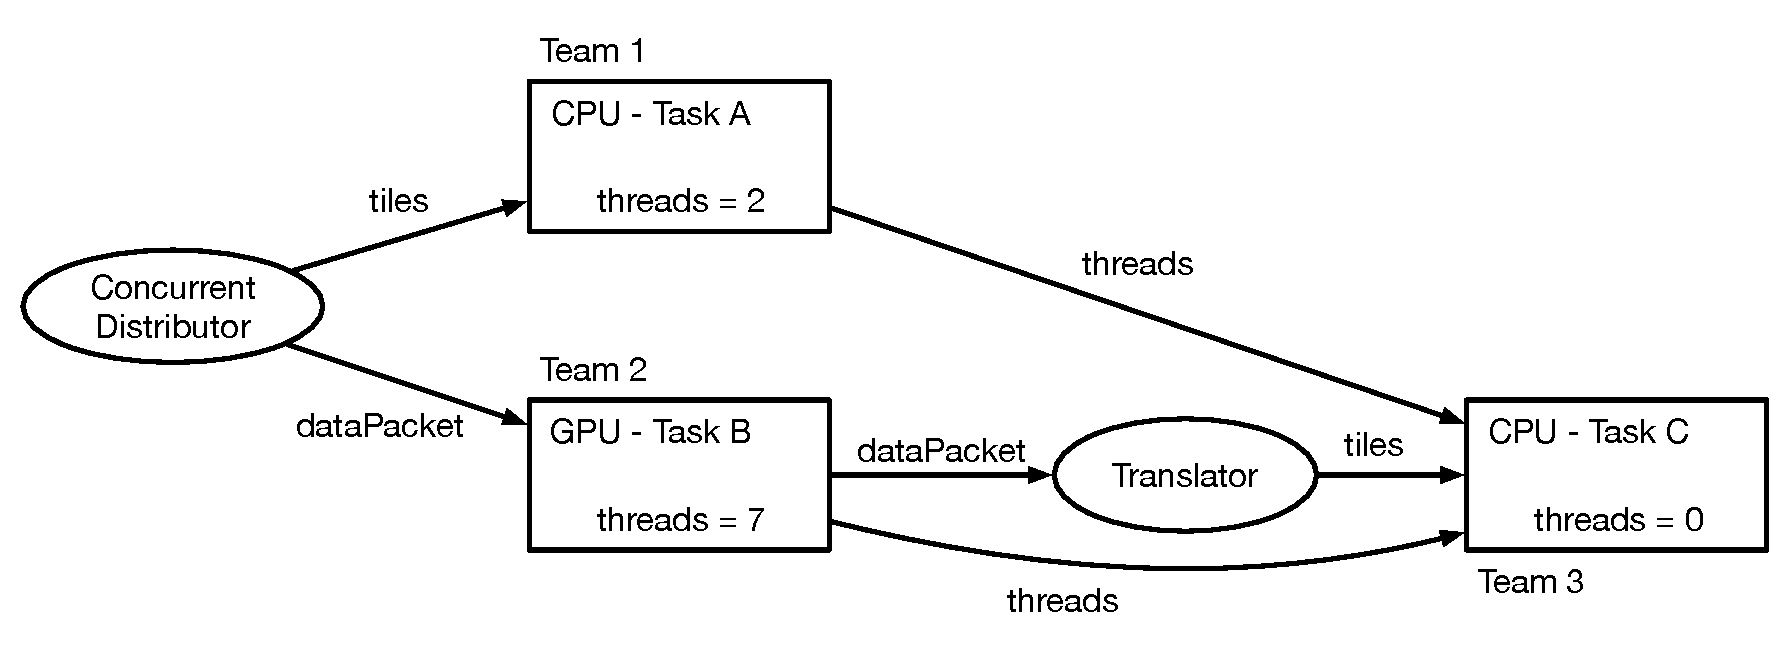
\includegraphics[width=5.5in]{ConcurrentItorExample.pdf}
\caption[]{\textcolor{red}{Add general information related to requirements.
Also specify the assumptions about RW independence of tasks so that these
topologies will give the correct results regardless of order of execution.}}
\label{fig:ConcurrentItor}
\end{center}
\end{figure}

\begin{figure}[!ht]
\begin{center}
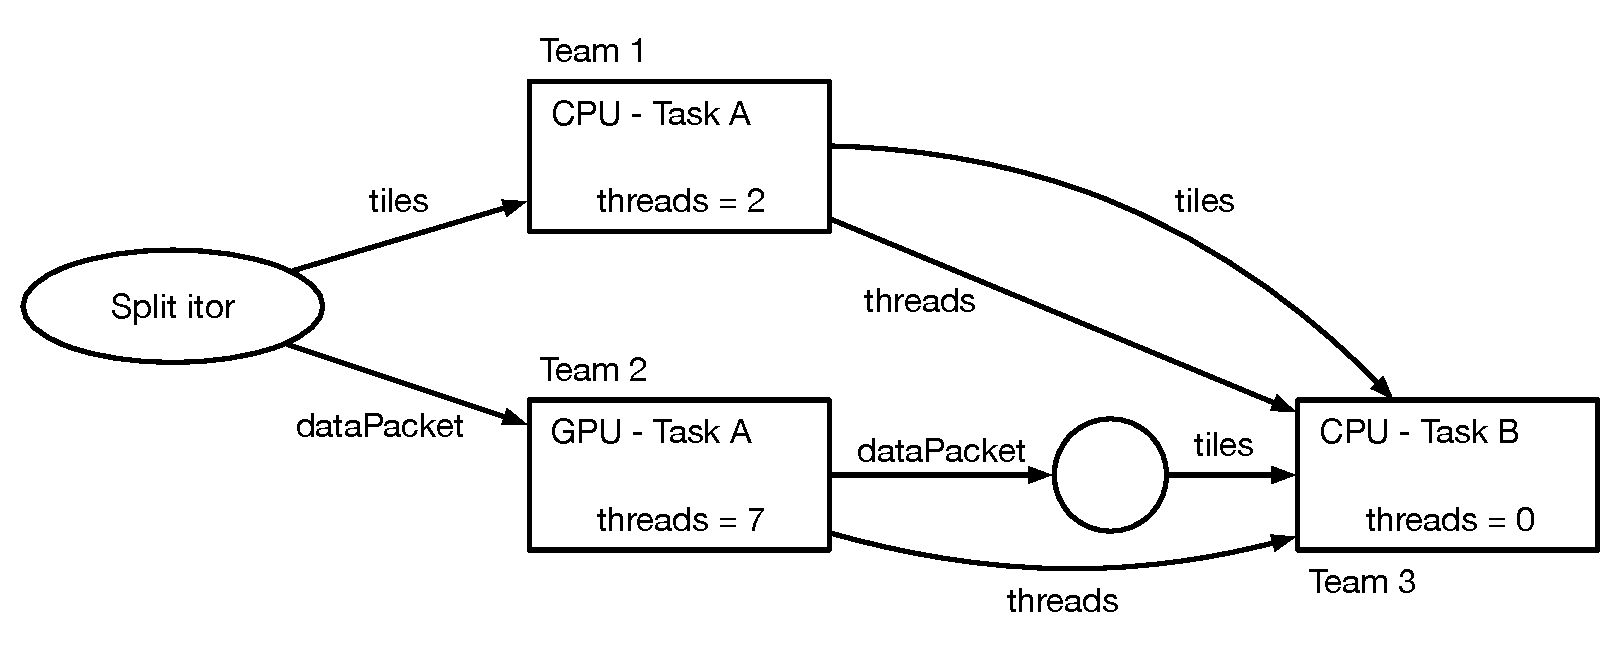
\includegraphics[width=5.5in]{WorkSplittingExample.pdf}
\caption[]{\textcolor{red}{Add general information related to requirements.
Also specify the assumptions about RW indepence of tasks so that these
topologies will give the correct results regardless of order of execution.}}
\label{fig:SplitItor}
\end{center}
\end{figure}

%%%%%----- RUNTIME TECHNICAL SPECIFICATIONS & DESIGN SECTION -----%%%%%
\section{Runtime Technical Specifications \& Design}
The statements that appear in this section are being referred to as technical
specifications rather than requirements in that these statements are low-level
and directly informed by the design and how we plan to implement the design.
Therefore, it is expected that a change in the design that does not violate the
above requirements could still require significant changes to the technical
specifications in this section.\\

One main intent of the technical specifications is to highlight \textit{some} of
the key ideas, difficulties, complexities, and subtleties that should be kept in
mind when studying and maintaining the code.  Also, use, corner, and edge cases
that have been identified are presented as motivation for technical
specifications.  Finally, some statements are made because the correctness of
the design and implementation require that they be satisfied.  For such
statements, proofs are given to explain how we know that the specification is
satisfied by the design and actual implemetation.

%%-- THREAD TEAMS SUBSECTION
\subsection{Thread Teams}
A thread team is fundamentally event-driven software and as such its design has
been specified as a finite state machine (FSM).  However, the behavior in a
given state cannot be specified solely by a single qualitative state variable.
Rather, the behavior will depend on a qualitative state variable, which is
called the mode, as well as the quantitative internal state variables $N_i, N_w,
N_c, N_Q$ that respectively keep track of 
\begin{itemize}
\item{the number of Idle threads in the team,}
\item{the number of threads that are Waiting for work to be added,}
\item{the number of threads applying a task on a unit of work, and}
\item{the number of units of work in the team's pending work queue.}
\end{itemize}
Note that the definitions of $N_i, N_w, N_c$ imply that each thread is
always in one and only one of the Idle, Waiting, and Computing states but that
this EFSM need not track the actual state of each thread --- it is only the
aggregated thread state information that is important.  Therefore, the runtime
is an extended finite state machine (EFSM)
\[
M = (Q, X, I, O, s_0, T)
\]
where
\begin{itemize}
\item{$Q$ is the finite set of qualitative modes,}
\item{$X = \set{(N_i, N_w, N_c, N_Q) \in \Z_{\ge 0}^4\,|\,N_i + N_w + N_c =
N_{max}}$ is the set of internal state variables where $N_{max}$ is the
number of threads in the team,}
\item{$I$ is the set of internal and external events,}
\item{$O$ is the set of outputs,}
\item{$s_0 = (q_0, x_0) \in Q \times X$ is the initial state, and}
\item{$T : Q \times X \times I \to Q \times X \times O$ is the transition
function that is evaluated by the EFSM at each occurrence of an event to
identify the output to be performed as well as the state to which the EFSM must
be transitioned.}
\end{itemize}

Note that the set of all possible states is not $Q \times X$.  There are
elements in that set that the EFSM must not occupy.  See
Specs~\ref{spec:Closed_NoWork} and~\ref{spec:NoMoreWork_NeedThread} for examples
of such prohibited states.  Therefore, the above specification of $T$ is only
correct if we assume that the output associated with such prohibited states is
to inform client code of an error so that the EFSM can be terminated.\\

The set $Q$ contains the modes
\begin{itemize}
\item{\TeamIdle --- all threads Idle and no work in the queue}
\item{\TeamRunningOpen --- a task has been given to the team and units of work
on which to apply the task can still be given to the team (\textit{i.e.} an
execution cycle has been started)}
\item{\TeamRunningClosed --- a task is being applied but no more units
of work can be given to the team in the current execution cycle}
\item{\TeamRunningNoMoreWork --- a task is being applied, no more
units of work can be given, and the team has identified that the task has
already been applied to or is currently being applied to all units of work given
to the team for the current execution cycle}
%\item{\TeamTerminating --- the client has indicated that it no longer needs the team.}
\end{itemize}

The set $I$ of events is the union of events triggered by clients through the
team's interface
\begin{itemize}
\item{\texttt{startTask} --- give the team a task and activate a given number of the
$N_{max}$ Idle threads in the team to work on it}
\item{\texttt{increaseThreadCount} --- activate a given number of Idle threads in the
team so that they can start working on the task as well}
\item{\texttt{enqueue} --- give the team a unit of work on which to apply its
task}
\item{\texttt{closeTask} --- indicate (without blocking the caller) to the team
that no more units of work will be given for the current task}
%\item{\texttt{$\sim$ThreadTeam} --- thread team no longer needed}
\end{itemize}
with the set of events triggered internally
\begin{itemize}
\item{\texttt{activateThread} --- wake an Idle thread so that it can participate
in applying a task to given units of work, look for pending work, and update its
state accordingly}
\item{\texttt{transitionThread} --- wake a thread that is Waiting for work so
that it can evaluate if there is pending work and update its state accordingly}
\item{\texttt{computationFinished} --- a Computing thread finished applying the team's
task to a unit of work and shall evaluate if there is pending work and update
its state accordingly}
%\item{\texttt{threadTerminated} --- emitted by a thread to indicate that it has
%terminated}
\end{itemize}

Note that \texttt{computationFinished} is different from the other events and it
is important to understand how it is different as well as how we define it to
make certain that this event does not break the rules of a FSM.  Specifically,
when a thread transitions to Computing it does not sleep or wait on another
event as is the case for Waiting or Idle threads.  Rather, it does work.  Seen
in this light, a state transition in the EFSM that results in a thread becoming
a Computing thread does not terminate until the Computing thread finishes
applying the team's task to its current unit of work.  Therefore, we should not
allow any other thread to alter the state of the EFSM until the work is
finished, which is not acceptable.\\

Therefore, we emphasize that in our design the Computing thread is
\textit{effectively} sleeping while it is applying the team's task to a unit of
work and a EFSM state transition can finish when such a thread ``goes to
sleep.''  It is sleeping not in the sense of no resource usage, but rather from
the perspective of not being an active member of the runtime infrastructure
while it is computing.  As with Waiting and Idle threads, the Computing threads
need to be awakened by a dedicated event, which is the
\texttt{computationFinished} event.  This event is ``emitted'' by a Computing
thread when it finishes applying a task to its current unit of work and can only
be received by the thread itself.\\

The initial state is defined to be
\[
s_0 = \left(q_0, (N_i, N_w, N_c, N_Q)_0\right) = \left(\TeamIdle, (0, 0, 0, 0)\right).
\]

The set $O$ and the transition function $T$ encapsulate the complexity of the
runtime and are specified in the spreadsheet XXX.  A state diagram for the team
that indicates only states and transitions is shown in
Figure~\ref{fig:TeamStateDiagram}.  A similar state diagram for threads in the
team is shown in Figure~\ref{fig:ThreadStateDiagram}.  These figures are
intended only to aid in understanding the design of the runtime.  The content of
XXX should be understood to be the actual design of the runtime.\\

The design and implementation philosophy of the EFSM was to emphasize
correctness and maintainability.  One important consequence was to create a
design that accounts for almost all\footnote{There are a few states,
transitions, and events that the EFSM \textit{must} avoid so that the EFSM
functions properly.  For such cases, proofs have been given to prove correctness
of the design.  A few examples of some prohibited states are given in
Specs~\ref{spec:Closed_NoWork} and~\ref{spec:NoMoreWork_NeedThread}} possible
states, transitions, and events even though it could be proven that some
states/transitions/events are precluded from happening by the design itself.
Therefore, our design/implementation is hopefully robust and not sensitive to
small design changes.  Also, the mental load associated with working with the
design is lower since we do not have the burden of proving and maintaining
proofs of impossible states/transitions/events.  This is especially important as
the implementation of the thread team cannot make strong assumptions about the
predictability of the order of execution of code and events, which increases the
complexity of such proofs.  This philosophy is ugly in that the code might,
without the developers' knowledge, carry out actions that it shouldn't.  It also
means that we have not completely understood the full behavior of the EFSM.

\begin{figure}[!ht]
\begin{center}
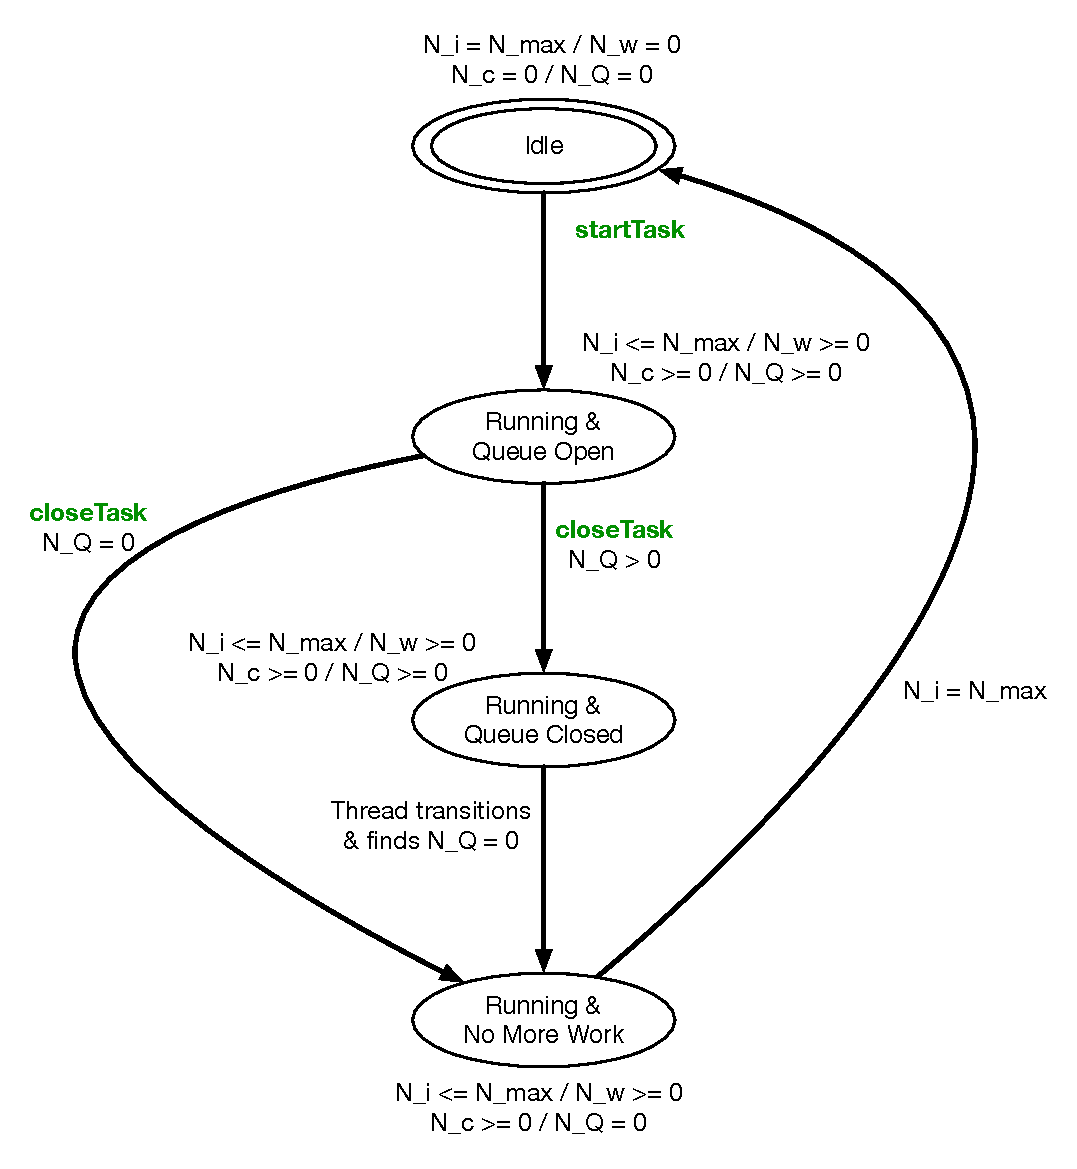
\includegraphics[width=5.0in]{TeamStates.pdf}
\caption[]{}
\label{fig:TeamStateDiagram}
\end{center}
\end{figure}

\begin{figure}[!hp]
\begin{center}
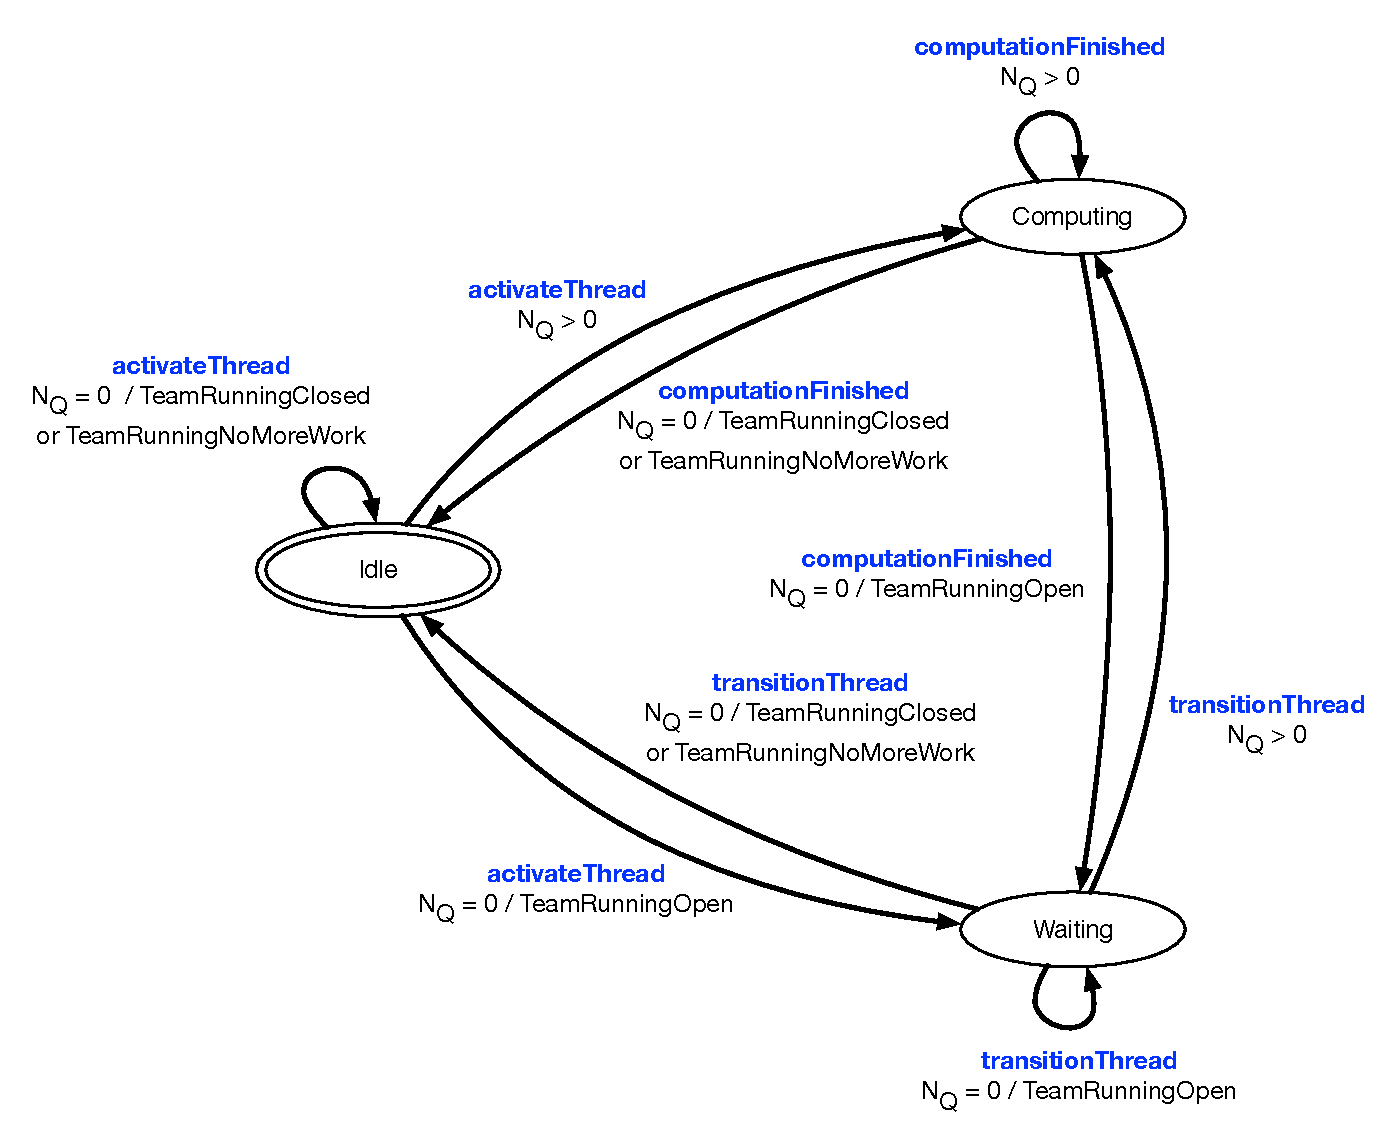
\includegraphics[width=6.5in]{ThreadStatesPersistent.pdf}
\caption[]{}
\label{fig:ThreadStateDiagram}
\end{center}
\end{figure}

\begin{spec}
\label{spec:Runtime_AtomicTransition}
As per the requirements of FSMs, each transition shall be implemented so that
the code executing the transition has sole access to the thread team's state
during the entirety of the transition.  This implies that no other thread can
alter the state simultaneously and that transitions are atomic.
\end{spec}
\textbf{Verification:}\hspace{0.125in}  Each thread team object has a single,
dedicated mutex that must be acquired to access or alter thread team state
information.  Each transition acquires the mutex either through an explicit
request or by a thread receiving an event.  The mutex is not released until
the transition is finalized.\\

Given the present implementation, it is important for transitions that
change the mode and emit internal signals that the code change the mode
\textbf{first} and then emit the signals.  This prevents the possible
(\textbf{TBC} for pthreads?) case that the signal is emitted and received before
the mode is correctly transitioned, which would violate
Spec~\ref{spec:Runtime_AtomicTransition} and cause the responding thread
to react to the signal is a way that is potentially not in accord with the true
mode of the EFSM.

\begin{spec}
A thread team shall maintain a set of pending units of work and all threads in a
thread team shall be able to check the set of pending units of work.  In
addition, each thread in the team shall be able to claim ownership of a single
unit of work by removing it from the set with the understanding that the thread
itself is responsible for applying the team's task to that unit of work.  It
shall be impossible for two threads to simultaneously claim ownership of the
same unit of work.
\end{spec}
\textbf{Verification:}\hspace{0.125in}  Pending work queues implemented as
stated.  As per Spec~\ref{spec:Runtime_AtomicTransition}, dequeueing of units of
work are only done after obtaining the mutex and no handle to dequeued units of
work remain.  Therefore, the only thread that can access a dequeued unit of work
is the thread that dequeued it.
\begin{spec}
All threads that transition to Idle must wait for the \texttt{activateThread}
event.  This includes threads in Idle that receive the \texttt{activateThread}
event but remain in Idle as well as all threads that are \textit{set} into the
Idle state when the EFSM is setup in the initial state.
\label{spec:IdleActivateThread}
\end{spec}

\begin{spec}
External code shall only be able to decrease $N_i$ through the
\texttt{startTask} and \texttt{increaseThreadCount} events and the runtime shall
be implemented such that a request to activate $i$ threads results in an error
if $i$ exceeds the number of Idle threads that are available for activation.
Note that this technical specification is consistent with
Req~\ref{req:ThreadBalance}.
\end{spec}
\textbf{Verification:}\hspace{0.125in}  In the present design, this requirement
is important because the runtime would emit more \texttt{activateThread} signals
than there are threads to receive them.  Because teams allow for thread
publishers/subscribers, undetected signals would amount to a loss of thread
resources at the level of the runtime.  Note that a thread-based implementation
will have a lag between when these events trigger the activation of Idle threads
and when these threads are actually activated.  The runtime design therefore
tracks the actual number of Idle threads with \texttt{N\_idle\_} = $N_i$ as well
as the number of threads pending activation with \texttt{N\_to\_activate\_}.
When a thread does receive \texttt{activateThread}, it decrements both
\texttt{N\_idle\_} and \texttt{N\_to\_activate\_} by one and increments by one
the internal state variable $N_i, N_w$ or $N_c$ corresponding to the thread's
next state.  To satisfy the requirement, both events throw an error if $i > $
\texttt{N\_idle\_} - \texttt{N\_to\_activate\_}.  No other public thread team
methods can emit \texttt{activateThread}.

\begin{spec}
\label{spec:Runtime_OneWait}
The interface of the thread team shall contain a \texttt{wait} method so that
for each task execution, the execution of an external thread that calls
\texttt{wait} is blocked until the termination of the task.  This interface
shall allow for at most one such thread to block its execution with this method
during each task execution.
\end{spec}
\textbf{Verification:}\hspace{0.125in}  Implemented a flag
\texttt{isWaitBlocking\_} to track if a thread has already called \texttt{wait}.

\textcolor{red}{Should we have a variant of wait that accepts a timeout?}

\begin{spec}
To maintain a simple design, client code shall only be allowed to attach and
detach thread subscribers when the team is in the {\TeamIdle} mode.  The same
requirement applies for work subscribers.
\end{spec}
\textbf{Verification:}\hspace{0.125in} Implemented directly as stated.

\begin{spec}
In the original designs, the Team state machine also contained a
{\TeamTerminating} mode.  The transition to this mode was allowed only from
{\TeamIdle} and was triggered by initiating the destruction of the team.  While
sensible, this design was flawed since a runtime error that occurs with the team
in any state could trigger the destruction of the team.  Therefore, the
termination of the EFSM and the clean-up of its resources shall be possible from
any state.
\end{spec}
\textbf{Verification:}\hspace{0.125in}  The destructor does not do any error
checking to confirm that destruction was called with the EFSM in any particular
state.  Also, the destructor assumes that there are Idle, Waiting, and Computing
threads at the time of calling.  For the Idle and Waiting threads, it signals 
them to terminate; Computing threads, it waits for them to finish their work and
discover that they should terminate.

\begin{spec}
\label{spec:Runtime_AwakenOnNoMoreWork}
All transitions to {\TeamRunningNoMoreWork} from a different mode shall awaken
all Waiting threads so that they can transition to Idle.
\end{spec}
\textbf{Verification:}\hspace{0.125in}  Implemented directly as stated.

\begin{spec}
\label{spec:Runtime_CompMustEnqueue}
Upon emitting/receiving the \texttt{computationFinished} signal, a Computing
thread shall enqueue the unit of work that it just finished applying the team's
task to with the team's work subscriber if the team has a work subscriber.
\end{spec}
\textbf{Verification:}\hspace{0.125in}  Implemented directly as stated.

\begin{spec}
\label{spec:Runtime_IdleOutput}
All transitions to {\TeamIdle} from a different mode shall
\begin{itemize}
\item{call the \texttt{closeTask} method of the team's work subscriber if it
has a work subscriber and }
\item{unblock the external thread that called \texttt{wait} if such a thread
exists.}
\end{itemize}
If the transition to {\TeamIdle} is handled by a Computing thread, then the
Computing thread shall enqueue its unit of work
(Spec~\ref{spec:Runtime_CompMustEnqueue}) prior to calling \texttt{closeTask}.
Note that this specification is not applicable to the case of \textit{setting}
the EFSM into its initial state.
\end{spec}
\textbf{Verification:}\hspace{0.125in}  Implemented directly as stated.

\begin{spec}
\label{spec:Runtime_IdleToIdle}
It is possible for an Idle thread to receive the \texttt{activateThread} event
when the team does not need threads to be activated (\textit{i.e.} the mode is
\TeamIdle \footnote{Consider a team that is both a thread publisher and
subscriber.  It is possible for the team to finish its work and transition to
{\TeamIdle} before its publisher and subscriber finish their work.} or
\TeamRunningNoMoreWork).  To avoid thread resource loss and to promote efficient
execution of the execution cycle's tasks, in this scenario the threads that
receive the unnecessary event shall remain in Idle and call
\texttt{increaseThreadCount(1)} for its thread subscriber if it exists.
\end{spec}
\textbf{Verification:}\hspace{0.125in} Implemented directly as stated.

\begin{spec}
\label{spec:Runtime_ForwardThreads}
To prevent thread resource loss at the level of the runtime, all threads that
transition to Idle shall call \texttt{increaseThreadCount(1)} of its thread
subscriber should it exist.  This specification is consistent with
Spec~\ref{spec:Runtime_IdleToIdle}, which could be understood to handle the
special case that an Idle thread transitions to Idle.  Note that this
specification is not applicable to the case of \textit{setting} the EFSM into
its initial state.  Note that this technical specification is consistent with
Req~\ref{req:ThreadSubPub}.
\end{spec}
\textbf{Verification:}\hspace{0.125in} Implemented directly as stated.

\begin{spec}
\label{spec:Runtime_NoEnqueue}
Client code shall only be allowed to give a team a unit of work if the team is
in the mode {\TeamRunningOpen}.  While the runtime could allow clients to give
units of work to a team that is in {\TeamIdle} with the understanding that the
work would be for the next task to be given to the team, there is no known use
case for which this is necessary.  Therefore, this specification is motivated by
the goal of simplifying the design.
\end{spec}
\textbf{Verification:}\hspace{0.125in}  The \texttt{enqueue} method is the only
means for giving a unit of work to a team.  Attempts to use this method when the
team is not in {\TeamRunningOpen} result in error.\\

Based on this specification, client code should call \texttt{startTask} on all
thread teams to be used on a task before enqueueing work with any of these.  This
practice will help avoid the case where an active work publisher tries to
enqueue work on a work subscriber that is still in the mode \TeamIdle.\\

As a final note, the design accounts for \texttt{transitionThread} events that
occur when no Waiting threads exist.  For each of these, this occurrence is
acceptable and no output is generated as part of the transition.  This
transition is included for the sake of completeness and can occur with the
current implementation when certain outputs broadcast \texttt{transitionThread}.
Unlike for \texttt{activateThread}, it is unimportant that there is no thread to
receive the event.  This is due to the fact that this event exists to inform a
Waiting thread to look for work or that it should determine that it should
transition to Idle.  If there are no Waiting threads because all threads are
Idle, then the team must be in \TeamIdle, in which case we don't need to
activate threads, or in \TeamRunningOpen.  In the latter case, we wait for
threads to be activated or for \texttt{closeTask} to be called to transition
the team to \TeamIdle.  If all threads are Computing, then these will discover
that there is pending work and the team will stay maximally busy.

%%-- TEAM IDLE SUBSECTION
\subsection{{\TeamIdle} State}
\begin{spec}
Similar to Spec~\ref{spec:Runtime_ForwardThreads}, if client code calls the
\texttt{increaseThreadCount} method of a thread team in \TeamIdle, the team shall
forward the pushed thread resources immediately on to its thread subscriber if
it exists.
\end{spec}
\textbf{Verification:}\hspace{0.125in}  Implemented directly as stated.

\begin{spec}
In the {\TeamIdle} mode, the queue shall always be empty with all threads in the
team in the Idle state.  This implies that no thread can be in the Waiting
state, the Computing state, or terminating and that all threads are therefore
(Spec~\ref{spec:IdleActivateThread}) waiting to receive the
\texttt{activateThread} event.
\end{spec}
\textbf{Verification:}\hspace{0.125in}  The initial state starts in {\TeamIdle}
and specifies that there is no work in the queue.  Also, all transitions to
{\TeamIdle} only happen if the queue is empty.  Therefore, the pending work
queue is always empty upon entry to \TeamIdle.  Finally, no work can be added to
the queue in the {\TeamIdle} state by Spec~\ref{spec:Runtime_NoEnqueue}.\\

The initial state specifies that all threads are Idle and transitions to
{\TeamIdle} only happen if the same is true.  Therefore, the claim is true upon
entry to {\TeamIdle} and all threads are waiting for \texttt{activateThread}.
Also, responses
\footnote{These cases are being considered should one of these
events be emitted when the team in not Idle, but is received after transitioning
to Idle.  With the current implementation, since all threads would be waiting on
\texttt{activateThread}, no threads would be waiting for the latter two events.}
to \texttt{activateThread}, \texttt{transitionThread}, and
\texttt{computationFinishes} do not transition the thread state and have the
responding threads wait for \texttt{activateThread}.  Therefore any attempt to
transition a thread terminates with the thread in Idle.

\begin{spec}
It would seem to be sensible to insist that an external thread cannot call
\texttt{wait} for a team that is in \TeamIdle.  However, it is possible that a
runtime execution cycle could finish and transition a team back to {\TeamIdle}
before an external thread has the chance to call \texttt{wait}.  Therefore, the
\texttt{wait} method shall be enabled in {\TeamIdle} and shall terminate immediately to avoid
unnecessary blocking of the calling thread.  Note that this does allow for
client code to superfluously call \texttt{wait} before the first execution cycle
is run and multiple times between cycles, both of which are logical errors.
\end{spec}
\textbf{Verification:}\hspace{0.125in}  Implemented directly as stated and in
accord with Spec~\ref{spec:Runtime_OneWait}.  

%%-- TEAM RUNNING & OPEN SUBSECTION
\subsection{\TeamRunningOpen}
\begin{spec}
It  would seem sensible to insist that an external thread cannot call
\texttt{wait} during a given execution cycle unless the \texttt{closeTask} event
has already been issued for the same cycle.  However, consider the case of two
teams, one of which is the work publisher for the other.  As per
Spec~\ref{spec:Runtime_IdleOutput}, when the publisher team transitions to
{\TeamIdle}, it calls the subscriber's \texttt{closeTask} method to inform the
subscriber that it will not be given more work.  This implies that the external
thread that triggers an execution cycle with the runtime does not know when
\texttt{closeTask} is called and therefore could call \texttt{wait} before this
event occurs.  Hence, a thread team in the state {\TeamRunningOpen} shall allow
for a thread to call \texttt{wait}.
\end{spec}
\textbf{Verification:}\hspace{0.125in}  Implemented directly as stated.

%%-- TEAM RUNNING & CLOSED SUBSECTION
\subsection{\TeamRunningClosed}
\begin{spec}
\label{spec:Closed_Transition}
If a team is in mode \TeamRunningClosed, then every thread that transitions to
Computing shall check if $N_Q = 0$ as part of the transition and after
dequeueing the unit of work on which it will apply its team's task.  If $N_Q =
0$, then during the same transition (and therefore before applying the task to
the dequeued unit of work) the thread shall change the mode to
\TeamRunningNoMoreWork.
\end{spec}
\textbf{Verification:}\hspace{0.125in}  A thread can be transitioned to
Computing from the Idle, Waiting, and Computing state.  If the mode is
{\TeamRunningClosed}, $N_Q = 1$, and a
thread receives any of the \texttt{activateThread}, \texttt{transitionThread},
or \texttt{computationFinished} events, then the induced transitions always changes
the mode to \TeamRunningNoMoreWork.  No other events result in decreasing $N_Q$
to zero in \TeamRunningClosed.

\begin{spec}
\label{spec:Closed_NoWork}
The transition from {\TeamRunningClosed} to \TeamRunningNoMoreWork, which is the
only transition possible for this mode, is triggered internally by the active
thread that dequeues the last unit of work (Spec~\ref{spec:Closed_Transition}).
Therefore, to avoid deadlock the design of the runtime shall be such that the
EFSM cannot be in mode {\TeamRunningClosed} with $N_Q = 0$.  Note that it is not
necessarily an error if $N_i = N_{max}$ in {\TeamRunningClosed} as the team
could be a thread subscriber and have a thread activated by its publisher so
that the team could eventually dequeue elements and determine that there is no
more work.
\textcolor{red}{Should each thread team store the pointer to its thread
publisher so that we can implement a rule here that if a team isn't a thread
subscriber and $N_i = N_{max}$, then we have an error?}
\end{spec}
\textbf{Verification:}\hspace{0.125in}  The only transition to
{\TeamRunningClosed} is from {\TeamRunningOpen}, which only occurs if $N_Q > 0$.
Hence, the specification is satisfied upon entry into the mode.  The value of
$N_Q$ can decrease in this mode only when a thread transitions to the Computing
state.   By Spec~\ref{spec:Closed_Transition}, the EFSM mode is transitioned to
{\TeamRunningNoMoreWork} as part of every transition that results in $N_Q = 0$.

%%-- TEAM RUNNING & NO MORE WORK SUBSECTION
\subsection{\TeamRunningNoMoreWork}
For the following, note that the only transitions into {\TeamRunningNoMoreWork}
are from {\TeamRunningOpen} and \TeamRunningClosed.

\begin{spec}
\label{spec:NoMoreWork_NoWork}
If a team is in \TeamRunningNoMoreWork, then it shall always be true that $N_Q =
0$.
\end{spec}
\textbf{Verification:}\hspace{0.125in}  
Since both transitions into {\TeamRunningNoMoreWork} only occur if $N_Q = 0$,
the specification is satisfied upon entry to the mode.  The only means to
increase $N_Q$ is by adding work \textit{via} \texttt{enqueue}, which is
prohibited in {\TeamRunningNoMoreWork} by Spec~\ref{spec:Runtime_NoEnqueue}.

\begin{spec}
\label{spec:NoMoreWork_TransitionToIdle}
If a team is in mode \TeamRunningNoMoreWork, then the last thread to transition
to Idle shall change the mode to \TeamIdle.  This transition is valid as $N_i =
N_{max}$ necessarily at the transition and by Spec~\ref{spec:NoMoreWork_NoWork}
it is certain that $N_Q = 0$.
\end{spec}
\textbf{Verification:}\hspace{0.125in}  If the transition to
{\TeamRunningNoMoreWork} is from \TeamRunningOpen, then $N_w > 0$ or $N_c > 0$
(to the contrary, $N_Q = 0$ and $N_i = N_{max}$ so that the transition is to
\TeamIdle).  If the transition is from \TeamRunningClosed, then it follows from
Spec~\ref{spec:Closed_Transition} that $N_c > 0$.  Therefore, upon entry to the
mode, there is at least one thread that could transition to Idle.  Since
satisfaction of Spec~\ref{spec:NoMoreWork_NoWork} implies that $N_Q = 0$, all
Computing threads will determine upon finishing the application of the team's
task to the current unit of work that there is no more work and will
subsequently transition to Idle.  Similarly, satisfaction of
Spec~\ref{spec:Runtime_AwakenOnNoMoreWork} implies that all threads in the Wait
state will be awakened, determine that there is no work, and transition to Idle
as well.  Therefore, all non-active threads will eventually transition to Idle.
Given this and the fact that the reception of \texttt{activateThread} events are
effectively ignored by Idle threads, we conclude that there will be a last
thread that transitions to Idle.  This thread is programmed to transition the
mode to \TeamIdle.

\begin{spec}
\label{spec:NoMoreWork_NeedThread}
The transition from {\TeamRunningNoMoreWork} to \TeamIdle, which is the only
transition out of this mode, occurs when the last non-Idle thread transitions to
Idle (See Spec~\ref{spec:NoMoreWork_TransitionToIdle}).  Therefore, to avoid
deadlock the design of the runtime shall prohibit the EFSM from being in a state
with {\TeamRunningNoMoreWork} and $N_i = N_{max}$.
\end{spec}
\textbf{Verification:}\hspace{0.125in} As shown in the Verification of
Spec~\ref{spec:NoMoreWork_TransitionToIdle},  $N_i < N_{max}$ upon entry to the
mode.  As $N_i$ can only decrease by at most one with each thread transition,
which are atomic (Spec~\ref{spec:Runtime_AtomicTransition}), satisfaction of
Spec~\ref{spec:NoMoreWork_TransitionToIdle} implies that $N_i$ cannot be set to
zero in {\TeamRunningNoMoreWork} without also simultaneously causing the mode to
change to \TeamIdle.  Hence, $N_i < N_{max}$ in {\TeamRunningNoMoreWork} up to
the transition to \TeamIdle.

\subsection{Possible Requirements}
%If a thread team is going to ship data to an accelerator like a GPU, then the
%unit of work for such a thread team shall be a data packet of tiles (with the
%possibility that the tiles are the trivial tiling).  This includes the
%possibility of data packets that consist of a single tile (and therefore tile
%that consist of a single block). 

%If a thread team is going to ship data to the host, then the unit of work for
%such a thread team shall be a tile (with the possibility that the tiles are the
%trivial tiling).

The queue thread shall create the iterator indicated to it by the parameters
passed to executeTask and shall be able to form all necessary units of work from
this.  This is too specific.  What if it can just queue tiles to every team and
the units of work are formed at dequeueing?  Who is responsible for the
shipments then?  Who is responsible for bringing data back?

%Consider a unit of runtime work that includes a GPU-concurrent task, a
%CPU-concurrent task, and a Post-concurrency CPU task in its task bundle.  Then
%for each block in a data packet, the concurrent CPU task will have blocks of
%input data (CC, FC[XYZ], Fluxes[XYZ], etc.), output data (CC, FC[XYZ],
%Fluxes[XYZ], etc.), and scratch blocks (e.g. grav[XYZ], auxC).  The concurrent
%GPU task will have the same, but non-intersecting block structure.  The
%post-concurrency CPU task can use whatever is in MFabs that is not being worked
%on by the concurrent CPU task and can allocate its own CPU scratch blocks.  We
%can get the CPU scratch memory through the runtime memory manager, but I don't
%know if we need to manage that memory or just let failures happen.  This assumes
%that the host memory will never be the limiting memory pool factor (i.e. that
%the host memory will always be much larger than the device memory).\\

%It is possible that certain units of runtime work will not need to bring the
%data back to the host memory as that same data is needed by the next runtime
%execution in the same device.  However, since we cannot assume that all the
%memory will fit in the device memory, we must assume that in the worst case only
%a fraction of the intended blocks will stay in the device memory.  The runtime
%shall maintain location information for each block that persists across calls to
%the runtime.  When the next runtime execution begins, those blocks already in
%the device shall be grouped into one or more data packets and work immediately
%launched on these.  The runtime shall not include these same blocks in a
%subsequent data packet so that we avoid repeated work.  FLASH shall abort
%execution if, at the end of a time step, we have blocks of persistent data
%(\textit{e.g.} unk) that are not in the host memory.  \textcolor{red}{Are these
%really requirements that we want?  If yes, then the blocks in the device memory
%would be the first data packet and therefore we get the pipeline up and running
%quicker.}  Example of this is unsplit Hydro.  The computeFluxes routine pulls in
%the UNK data on CC1 and updates the fluxes.  Neither needs to go back to the GPU
%ever.  The updated solution is in CC2.  Note that if we have the future case of
%host and some devices sharing the same physical memory, this requirement could
%become more imporatant.  Therefore, giving the runtime more parameters to inform
%data movements could be important.\\

\end{document}
